Differential equations allow us to describe the rate of change of quantities over time. They are used widely throughout engineering --- for instance when modelling fluids, electromagnetic radiation and the motion of rigid bodies. This worksheet introduces a type of differential equation called ordinary differential equations, with a particular emphasis on finding unique solutions to such equations. Let's first recap some of the key definitions from the lectures.\\

{\bf Recap}\\
Differential equations are made up of independent and dependent variables.
\begin{enumerate}
 \item {\em Independent variables} do not depend on any other variables, usually appearing at the bottom of differentials.
 \item {\em Dependent variables} depend on other variables, usually appearing at the top of differentials.
 \end{enumerate}
An {\em ordinary differential equation} (ODE) is a differential equation with only one independent variable. Denoting the independent variable as $t$ and the dependent variable as $x$, an ODE can look something like this:
\begin{equation*}
 \frac{\dd x}{\dd t}=f(x,t).
\end{equation*}
A solution to this ODE will give $x$ as a function of $t$ and therefore can be written as $x(t)$. An ODE will not have a unique solution, but instead will admit a set of solutions. To make this clear, let's consider an example.\\

        \begin{center}
        
\includegraphics[scale=0.35]{rabbit.pdf}
        \end{center}
Imagine that a population of rabbits lives in a rabbit utopia --- a boundless island of endless grass with no predators. The rate at which the number of rabbits increases will be proportional to the number of rabbits. This is because if the number of rabbits becomes larger, there will be more rabbits breeding and so the rabbit population will grow at a faster rate. Suppose that the rate of change of our particular rabbit population can be described by the following ODE
\begin{equation}\label{eq:rabbit}
 \frac{\dd N}{\dd t}=4 N
\end{equation}
where $N$ is the number of rabbits and $t$ is the time in years. Here the number of rabbits $N$ is dependent on the time $t$, so $N$ is our dependent variable and $t$ is our independent variable. Therefore a solution $N(t)$ will give the number of rabbits as a function of time.

We can solve this equation by the technique of {\em separation of variables}. Separating the terms involving $N$ and the terms involving $t$s and integrating both sides we have
\begin{equation*}
 \int \frac{1}{N} \:\dd N = \int 4\:\dd t \implies \ln{N} = 4t + C.
\end{equation*}
Taking the exponential of both sides gives the solution
\begin{equation*}
 N(t)=A\text{e}^{4t}\hspace{10pt}\text{where}\hspace{10pt} A=\text{e}^{c}.
\end{equation*}
We can verify that this is a solution to our ODE for the rabbit population by simply substituting it in to \eqref{eq:rabbit}. Explicitly for the LHS we have
\begin{equation*}
 \frac{ \dd N(t)}{\dd t} = 4A\text{e}^{4t}\hspace{10pt}\text{and for the RHS we have}\hspace{10pt}4N(t)=4A\text{e}^{4t}.
\end{equation*}
Note that our solution satisfies the ODE for {\em any} real number $A$. So we have an infinite set of solutions for the ODE \eqref{eq:rabbit} given by
\begin{equation}\label{eq:gensol}
 x(t)= A\text{e}^{4t} \hspace{15pt}\text{where}\hspace{10pt} A \in \mathbb{R}.
\end{equation}
Four example solutions from the infinite solution set are plotted below.
        \begin{center}
        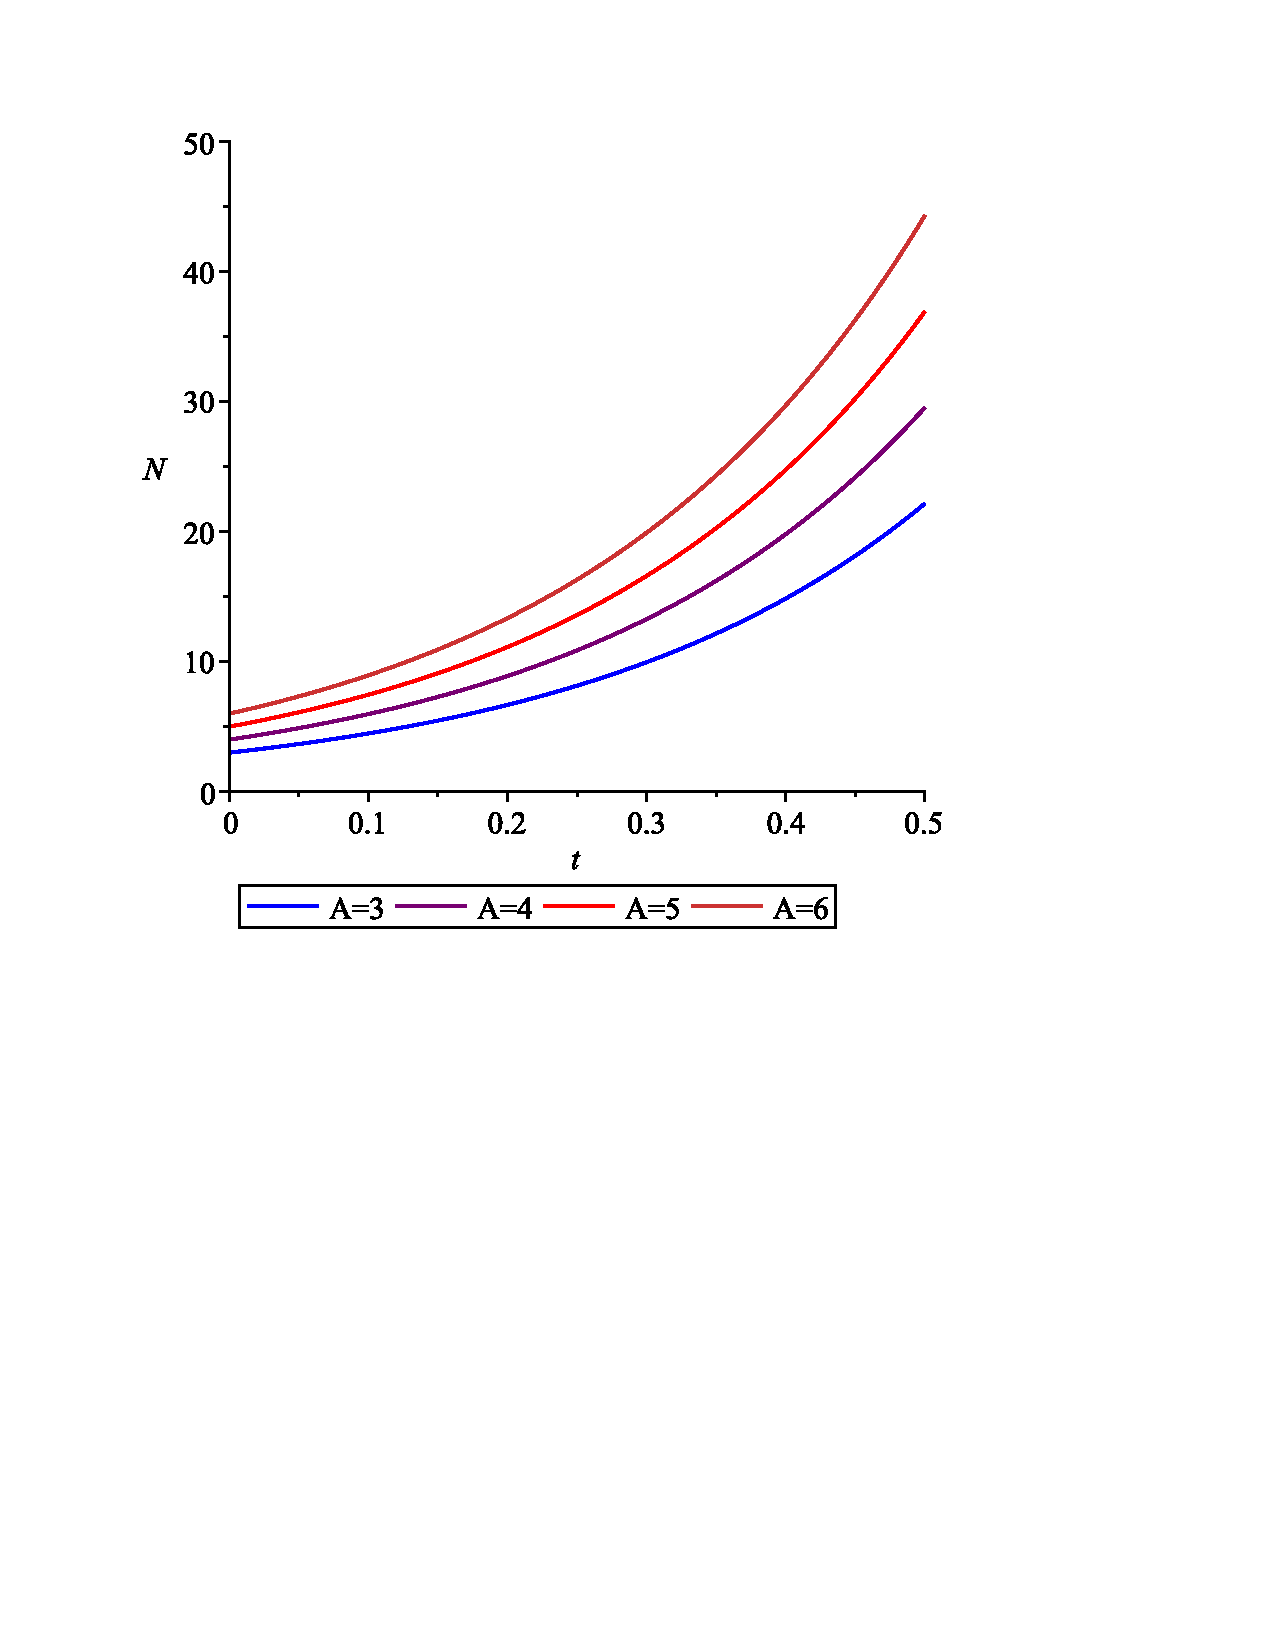
\includegraphics[scale=0.6]{sols-crop.pdf}
        \end{center}

So far as our ODE \eqref{eq:rabbit} only gives information on how fast the rabbit population is changing we do not yet have enough information to determine the number of rabbits at a given time. However, now suppose we know that at the beginning of year zero there were exactly six rabbits on the island. We can write this condition as 
\begin{equation}\label{eq:rabbit_ic}
 N(0)=6.
\end{equation}
This is called an {\em initial condition}. Together the initial condition \eqref{eq:rabbit_ic} and the ODE \eqref{eq:rabbit} make up an {\em initial value problem}. Under certain conditions, it is possible to obtain a unique solution for an initial value problem. For the rabbit example we have
\begin{equation*}
 N(0)=A\text{e}^{0}=6 \implies A=6
\end{equation*}
and so the solution to our initial value problem is
\begin{equation*}
 N(t)=6\text{e}^{4t}.
\end{equation*}
A solution like this that solves a specific initial value problem is known as a {\em particular solution}.

{\bf Quick Warm-up Exercise}
\begin{enumerate}
 \item The particular solution to the initial value problem we have just solved is shown in the graph above. Which line is it?
 \item Which line represents the solution to the initial value problem given by $N(0)=3$ and \eqref{eq:rabbit}? In this case how many rabbits will be on the island after six months?
 \item Which line represents the solution to the initial value problem given by $N(\ln({3})/4)=15$ and \eqref{eq:rabbit}?
\end{enumerate}

The {\em general solution} of an ODE satisfies the ODE for arbitrary initial conditions. So is \eqref{eq:gensol} the general solution to our ODE \eqref{eq:rabbit}? Well suppose we have some number of rabbits, say $N_{0}$, after some time, say $t_{0}$ years. Then
\begin{equation*}
 N_{0}=A\text{e}^{t_{0}} \implies A = \frac{N_{0}}{\text{e}^{4t_{0}}}
\end{equation*}
Because we can fix $A$ for {\em any} initial condition, \eqref{eq:gensol} is the general solution and the corresponding particular solution to any initial value problem is {\em unique}. We will discuss the uniqueness of different initial value problems later on in the worksheet.

Now for some questions...